\documentclass{article}
\usepackage{graphicx} % Required for inserting images
\usepackage{ctex}%使用中文
\usepackage{hyperref}%使用超链接
\usepackage{listings}%可以使用lstlisting命令

%\usepackage[fleqn]{amsmath}

\title{Git使用教程}
\author{apxl}
\date{\zhtoday}

\begin{document}

\maketitle

\section{前言之版本控制}

\href{https://mp.weixin.qq.com/s/Bf7uVhGiu47uOELjmC5uXQ}{视频文案}
\href{https://www.bilibili.com/video/BV1PG411L7of/?spm_id_from=333.788&vd_source=355508b521fc8e6490c52cd173d7b758}{另一个视频}

版本控制(Revision control)是一种在开发的过程中用于管理我们对文件、目录或工程等内容的修改历史,方便查看更改历史记录,追踪和记载一个或者多个文件的历史记录。

无论是工作还是学习,或者是自己做笔记,都经历过这样一个阶段,如图\ref{1.1}所示,我们就迫切需要一个版本控制工具:

\begin{figure}\label{1.1}
    \centering    
    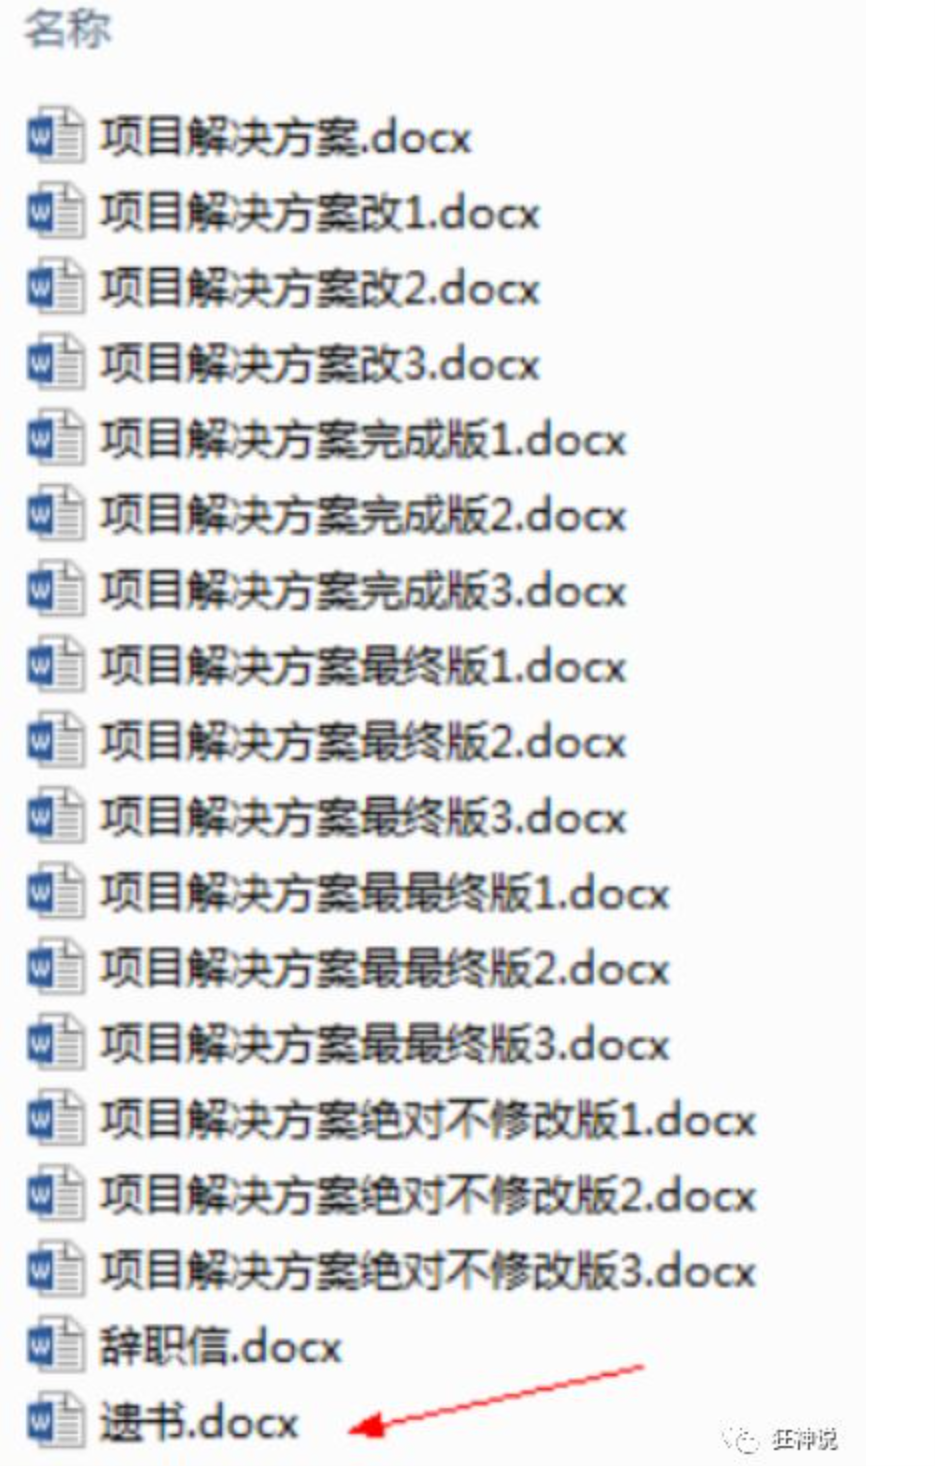
\includegraphics[width=\textwidth,keepaspectratio]{image/图片1.png}
    \caption{解决方案}
    %\label{1.1}
\end{figure}
%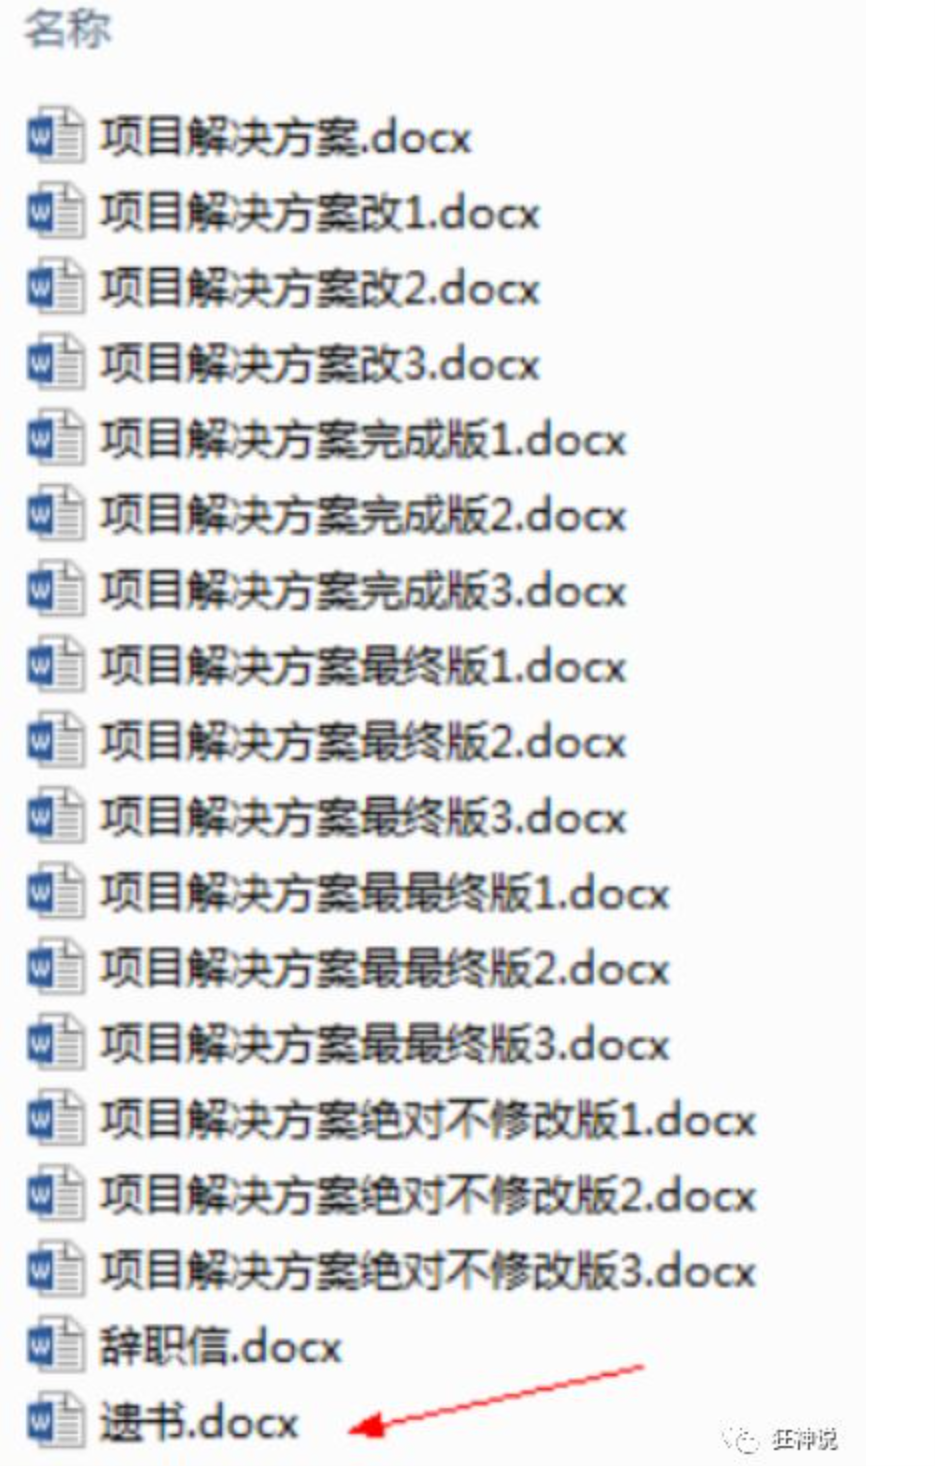
\includegraphics[width=\textwidth]{image/图片1.png}

\section{版本控制分类}

二者都是版本控制器,还有Perforce、Rational ClearCase、RCS等控制工具,但这两个更广泛:

版本控制分类:
\begin{enumerate}
    \item 本地版本控制:RCS,记录文件每次的更新,可以对每个版本做一个快照,或是记录补丁文件,适合个人用:
    
\centering
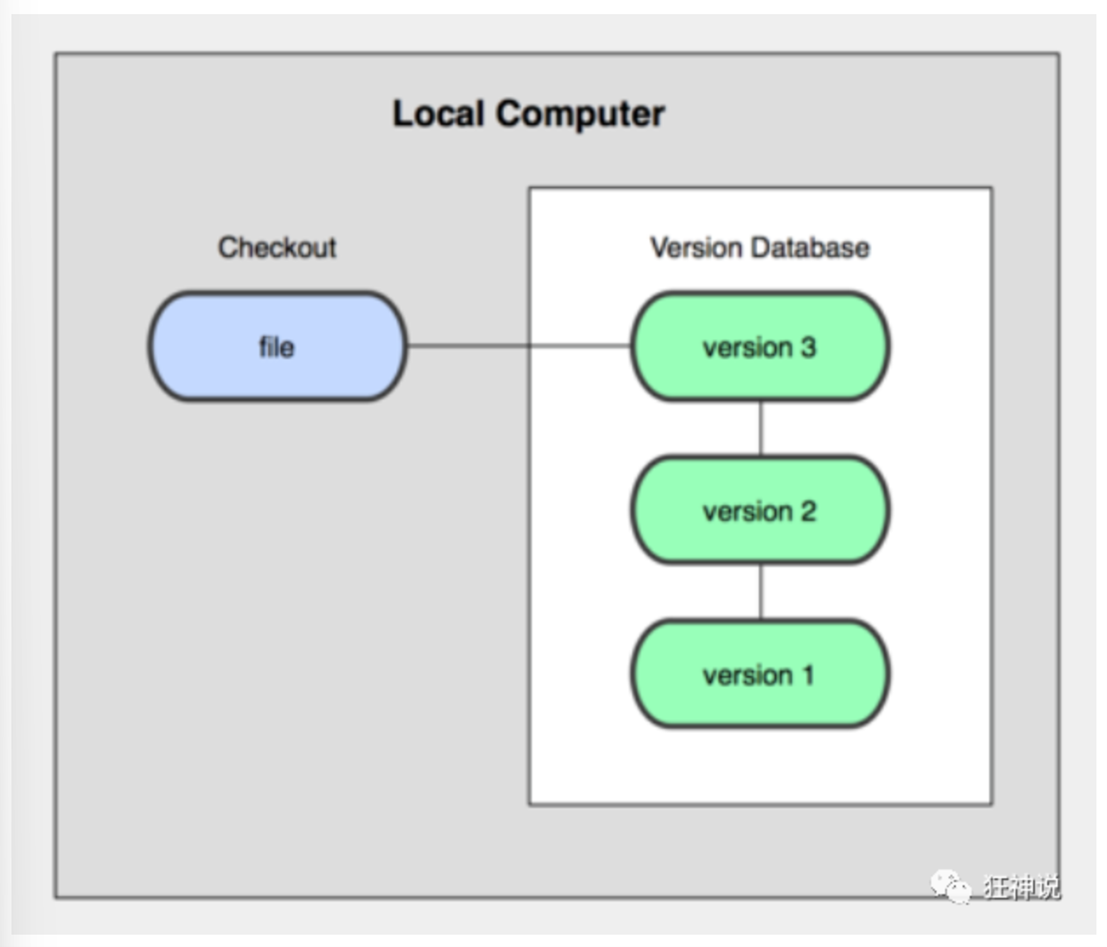
\includegraphics{image/2.1.png}

    \item 集中版本控制:SVN,所有的版本数据都保存在服务器上,协同开发者从服务器上同步更新或上传自己的修改,不太好,如果不连网的话,用户就看不到历史版本,也无法切换版本验证问题,或在不同分支工作:

\centering
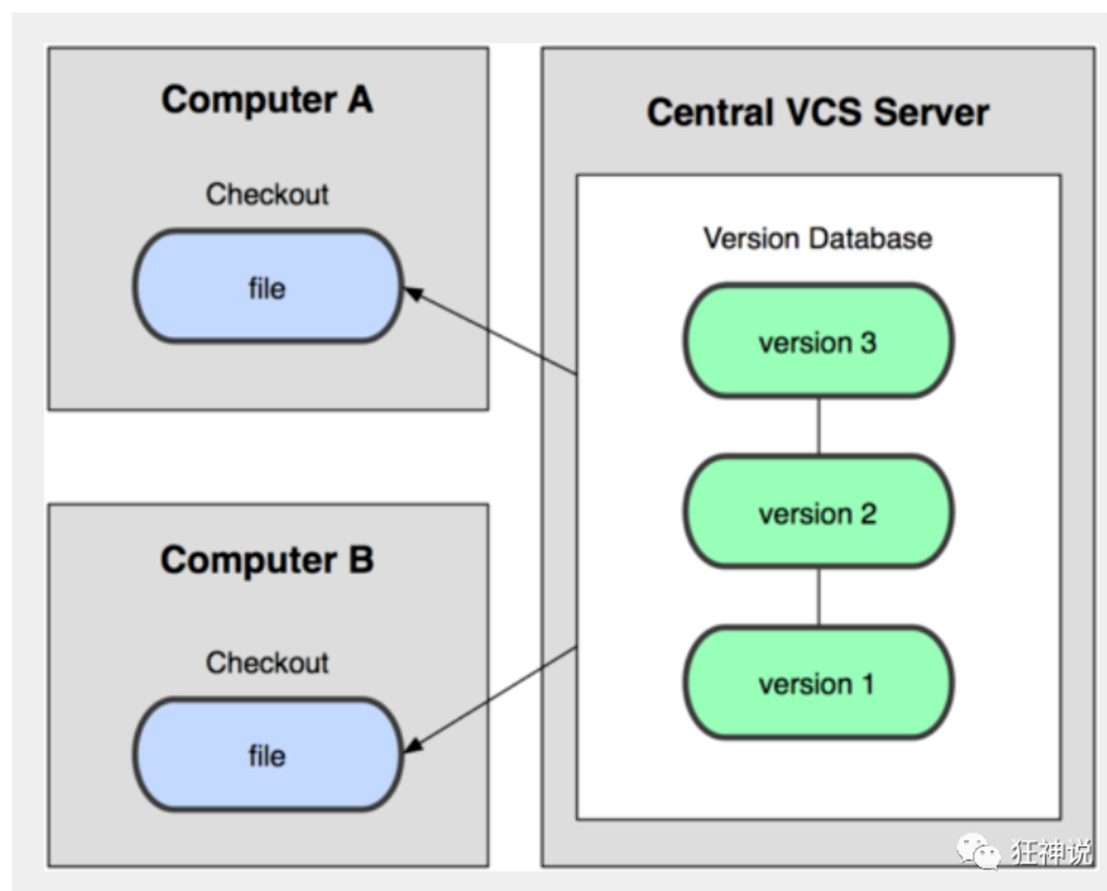
\includegraphics{image/2.2.png}

    \item 分布式版本控制:Git,所有版本信息仓库全部同步到本地的每个用户,这样就可以在本地查看所有版本历史,每个人都有全部代码:

\centering
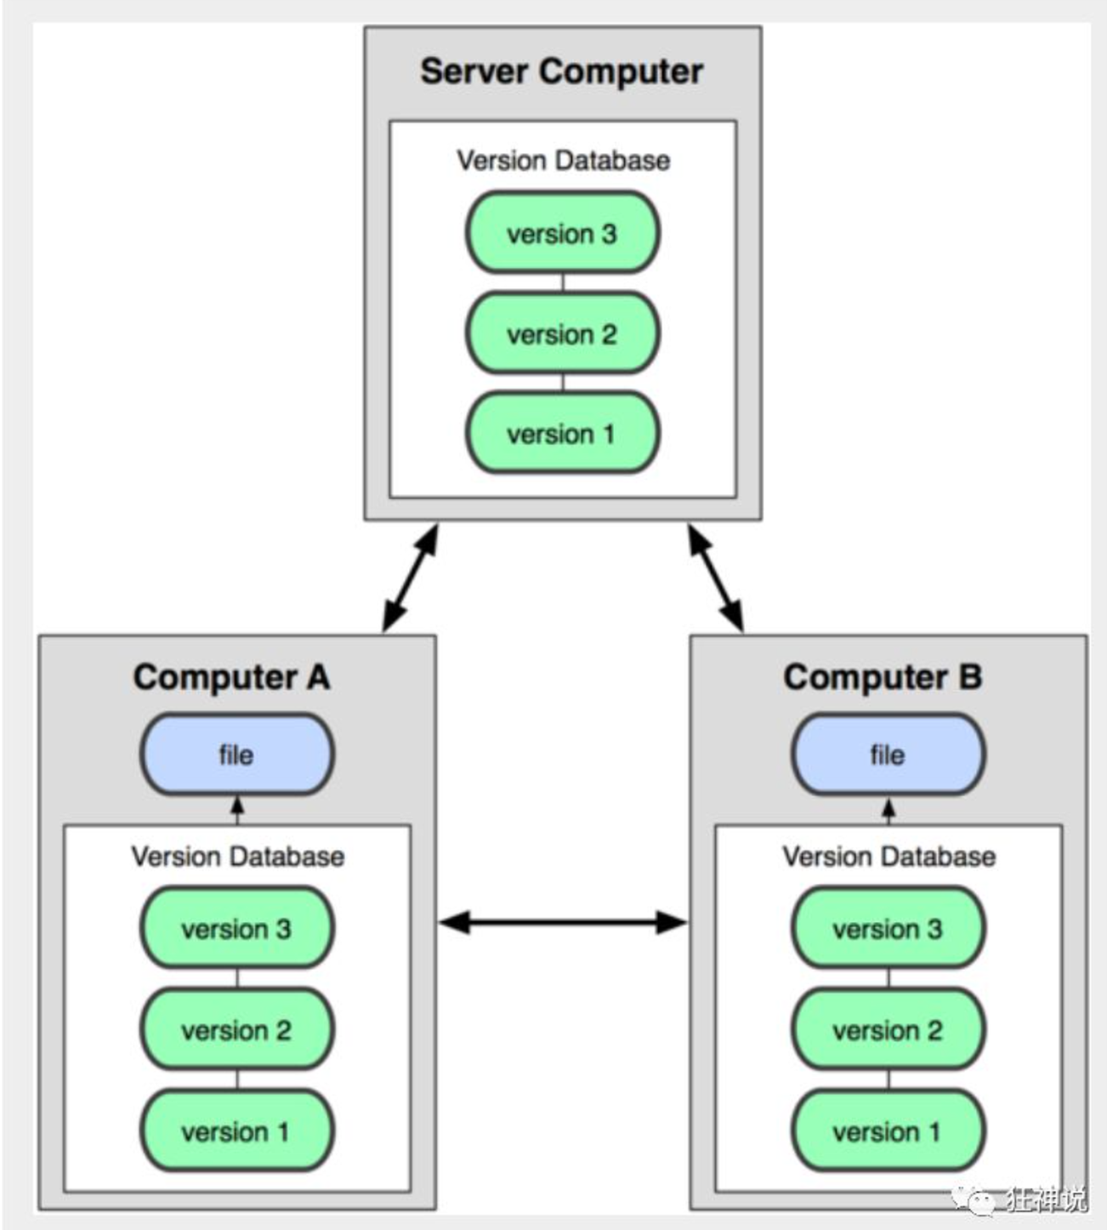
\includegraphics{image/2.3.png}

\end{enumerate}

\section{Git的历史}

Linux和Git之父李纳斯·托沃兹(Linus Benedic Torvalds).

Linux 内核开源项目有着为数众广的参与者。绝大多数的 Linux 内核维护工作都花在了提交补丁和保存归档的繁琐事务上(1991-2002年间)。到 2002 年,整个项目组开始启用一个专有(付费)的分布式版本控制系统 BitKeeper 来管理和维护代码。

到了 2005 年,开发 BitKeeper 的商业公司同 Linux 内核开源社区的合作关系结束,他们收回了 Linux 内核社区免费使用 BitKeeper 的权力。这就迫使 Linux 开源社区(特别是 Linux 的缔造者 Linus Torvalds)基于使用 BitKeeper 时的经验教训,开发出自己的版本系统。(2周左右!) 也就是后来的 Git!

\section{安装Git及环境配置}

\href{https://git-scm.com/download/win}{官网下载},下载对应的版本即可安装,无脑下一步即可,安装完毕就可以使用了:

安装成功后在开始菜单中会有Git项,菜单下有3个程序:

\centering
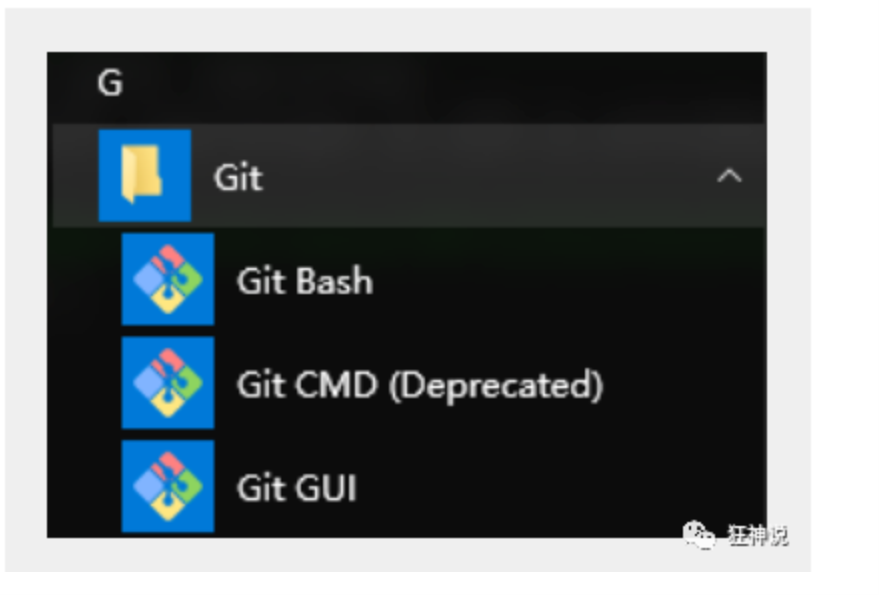
\includegraphics{image/4.1.png}
\begin{flushleft}
Git Bash:Unix与Linux风格的命令行,使用最多,推荐最多

Git CMD:Windows风格的命令行

Git GUI:图形界面的Git,不建议初学者使用,尽量先熟悉常用命令  
\end{flushleft}


\section{常用的Linux命令}
  
\begin{enumerate}
\renewcommand{\labelenumi}{\arabic{enumi}.}%改变序号,我这个没变
    \item cd..:回退到上一个目录
    \item cd +目录:进入指定目录
    \item pwd:显示当前所在的目录路径
    \item clear:清屏(命令行的),或者ctrl+L
    \item ls(ll,英文字母L的小写):都是列出当前目录中的所有文件,只不过ll(两个ll)列出的内容更为详细
    \item touch:新建一个文件,如touch index.js就会在当前目录下新建一个index.js文件
    \item rm:删除一个文件,rm index.js就会把index.js文件删除
    \item mkdir:新建一个目录,就是新建一个文件夹
    \item rm -r:删除一个文件夹, rm -r src 删除src目录
    \item mv:移动文件, mv index.html(目标文件) text(要移动的地方)
    \item history:查看命令历史
    \item exit:退出
\end{enumerate}

\section{Git的配置}
\begin{flushleft}%部分左对齐
所有的配置文件,其实都保存在本地。

查看配置:git config -l

查看系统:git config --system --list(在\verb|Git\etc\gitconfig|里面)
\end{flushleft}

\centering   
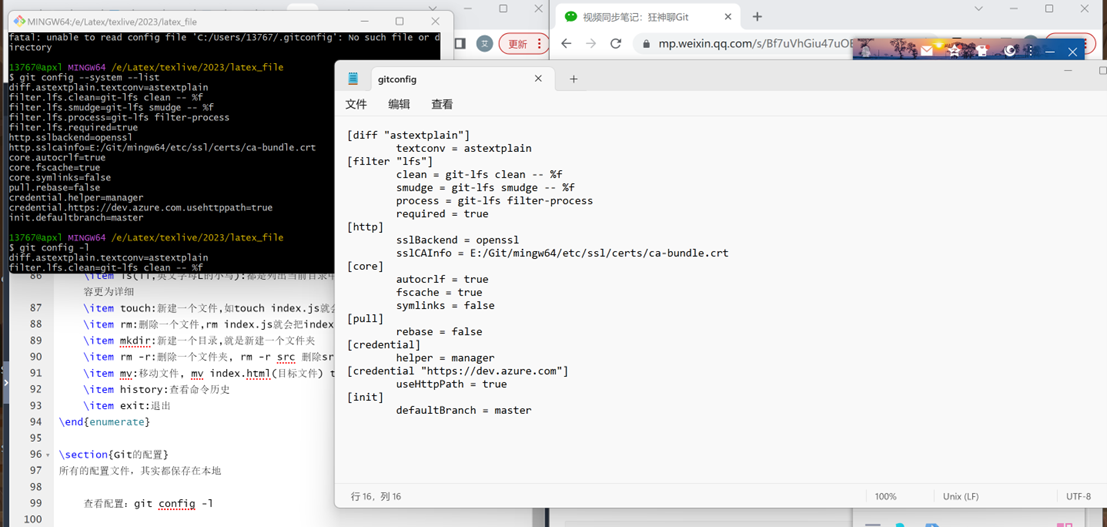
\includegraphics{image/6.1.png}
\begin{flushleft}
查看当前用户(global)配置:
\begin{lstlisting}
git config --global --list(在C:\Users\Administrator\ .gitconfig里面), 
\end{lstlisting}
git config --global --list(在\verb|C:\Users\Administrator\ .gitconfig|里面),此时应该是空的,必须要自己设置用户名和邮箱:
    
\begin{lstlisting}
    git config --global user.name "jiazhe"  #名称
    git config --global user.email 1376743525@qq.com   #邮箱
\end{lstlisting}
    写完后长这样:
\end{flushleft}

\centering
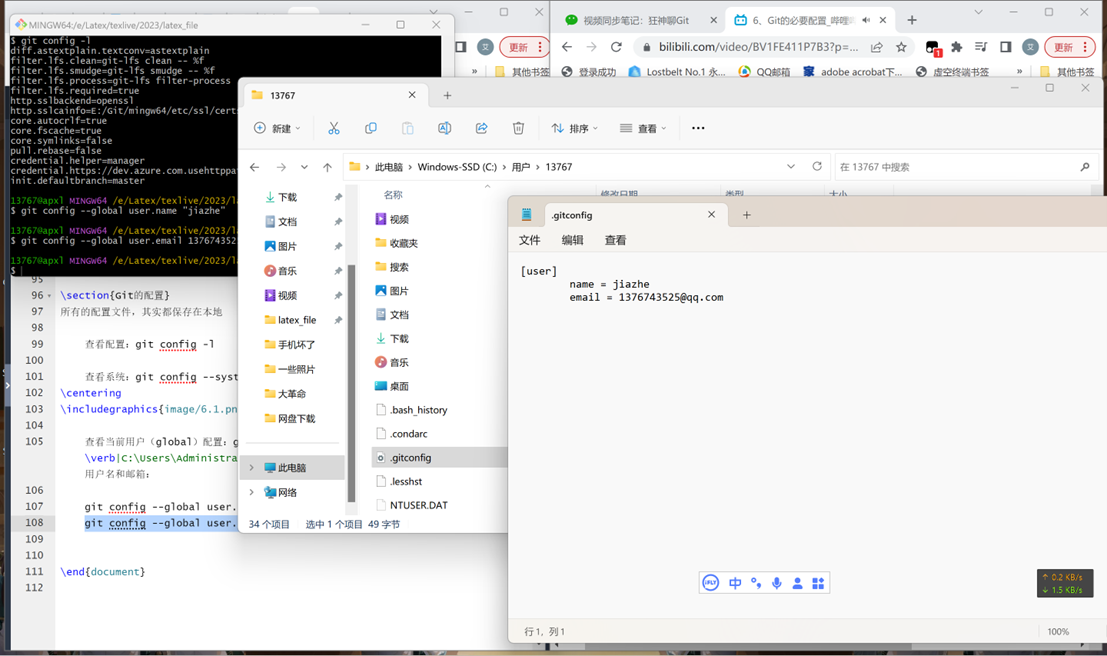
\includegraphics{image/6.2.png}

\section{Git的工作原理}
Git本地有三个工作区域:工作目录(Working Directory)、暂存区(Stage/Index)、资源库(Repository或Git Directory)。如果在加上远程的git仓库(Remote Directory)就可以分为四个工作区域:

\begin{itemize}
    \item Workspace:工作区,写代码的地方
    \item Index / Stage:暂存区,字面意思,一个隐藏文件
    \item Repository:仓库区(或本地仓库),字面意思,本地储存代码的地方
    \item Remote:远程仓库,托管代码的服务器,像github那样的应用
\end{itemize}

\centering
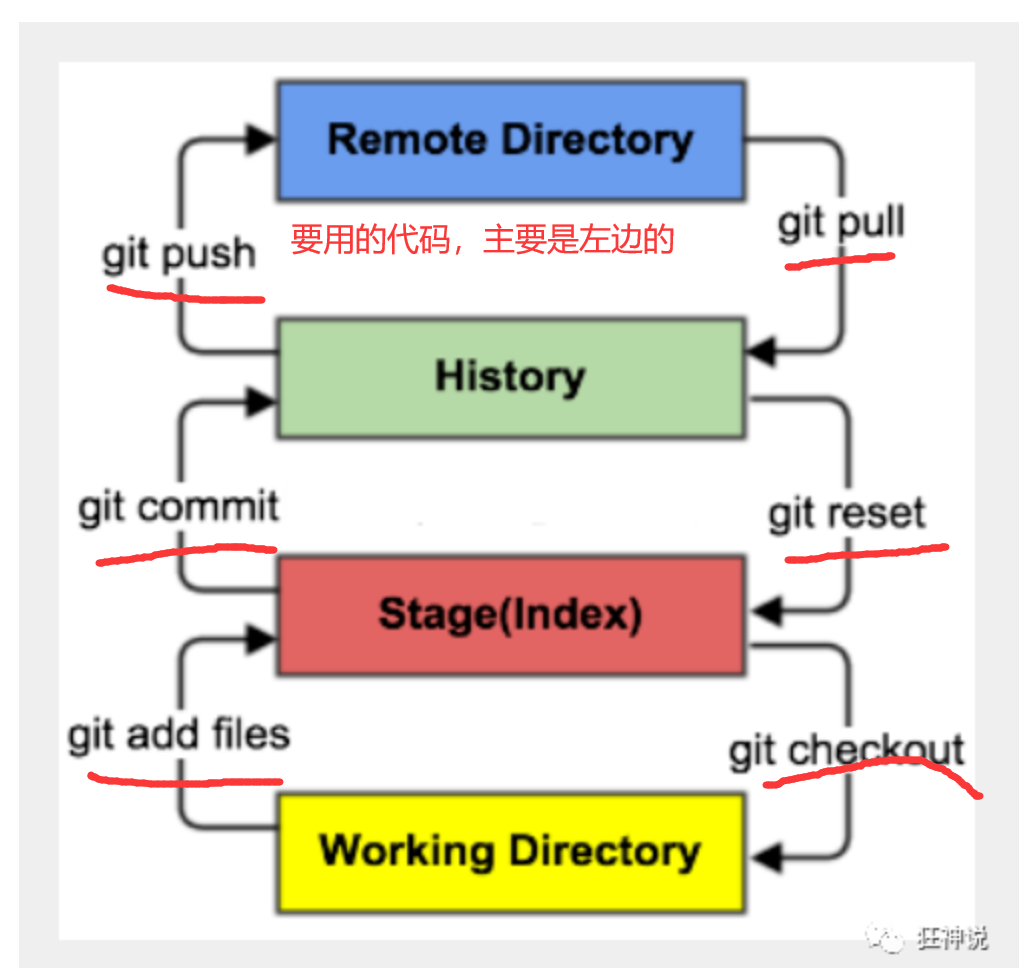
\includegraphics{image/7.1.png}

git的工作流程:
\begin{enumerate}
    \item 在工作区添加、修改文件
    \item 将需要进行版本管理的文件放入暂存区:git add .(表示将全部文件放入)
    \item 将暂存区的文件提交到仓库区:git commit
    \item 可选:将文件发送入远程应用:git push
\end{enumerate}

\section{Git项目创建及克隆}
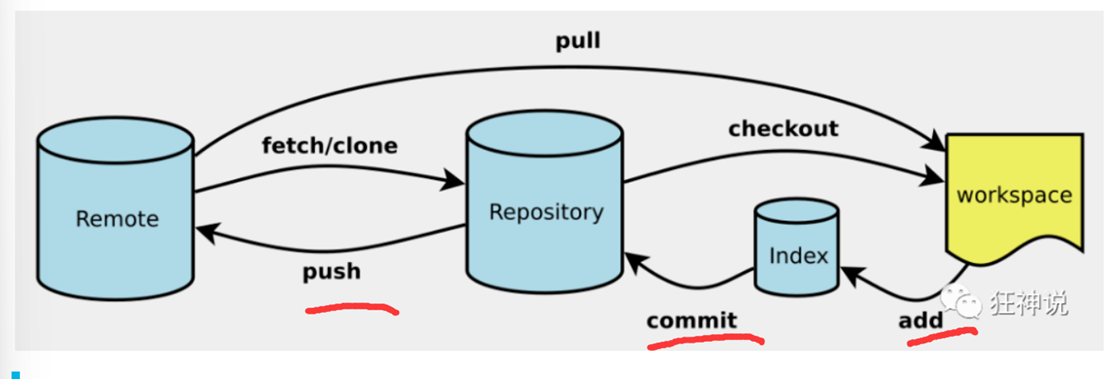
\includegraphics{image/8.1.png}

本地仓库搭建:
\begin{enumerate}
    \item 创建新的仓库:用GIT管理的项目的根目录执行git init命令:

    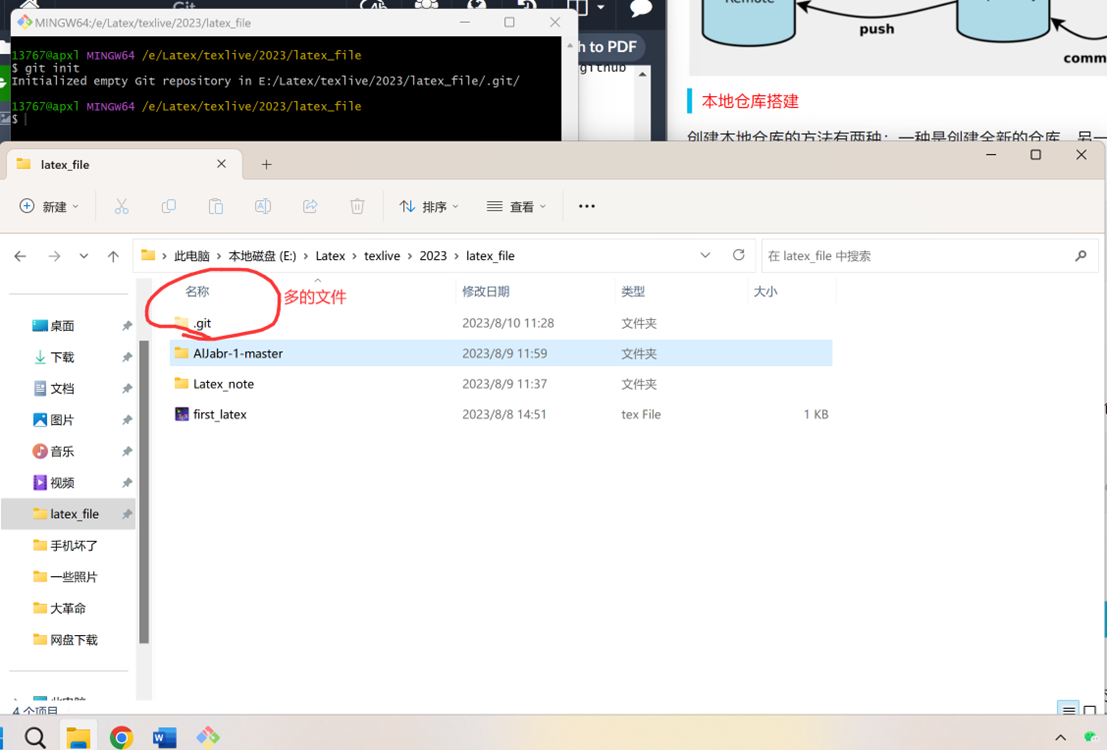
\includegraphics{image/8.2.png}

    \item 克隆远程仓库:github有一个专门提供克隆的链接,复制过来:git clone 网页(粘过来的那个)

    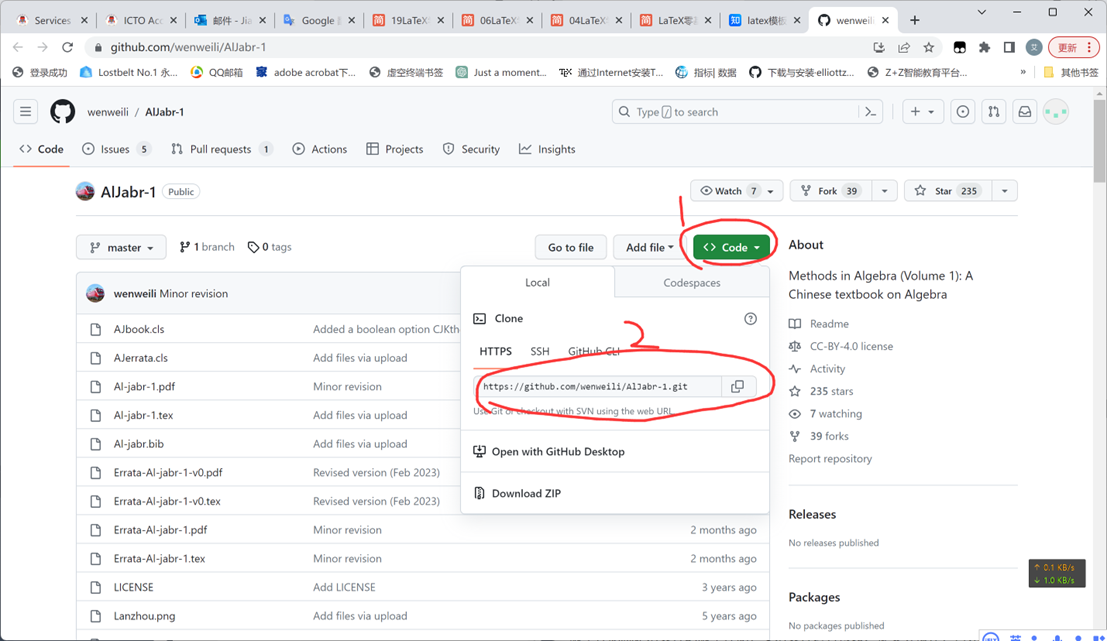
\includegraphics{image/8.3.jpg}
    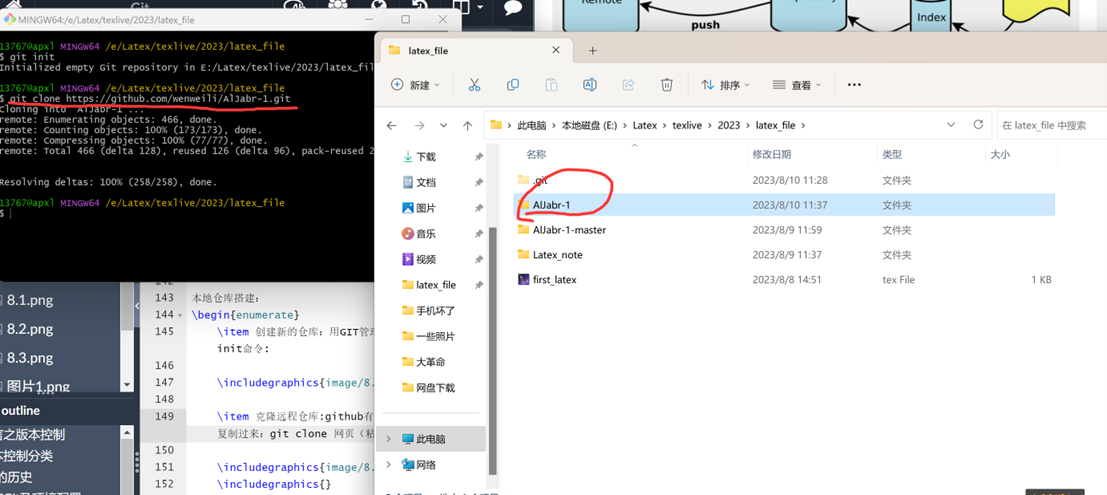
\includegraphics{image/8.4.jpg}  
\end{enumerate}

\section{Git的基本操作命令}
文件的四种状态:
\begin{itemize}
    \item Untracked: 未跟踪,此文件在工作区中, 但并没有加入到git库,通过git add 状态变为Staged,在暂存区
    \item Unmodify: 文件已经入库, 未修改
    \item Modified: 文件已修改, 仅仅是修改, 并没有进行其他的操作
    \item Staged: 暂存状态,文件在暂存区,执行git commit则将修改同步到仓库区中
\end{itemize}
查看文件状态:git status [filename]

查看所有文件状态:git status

第一次用是这样的:
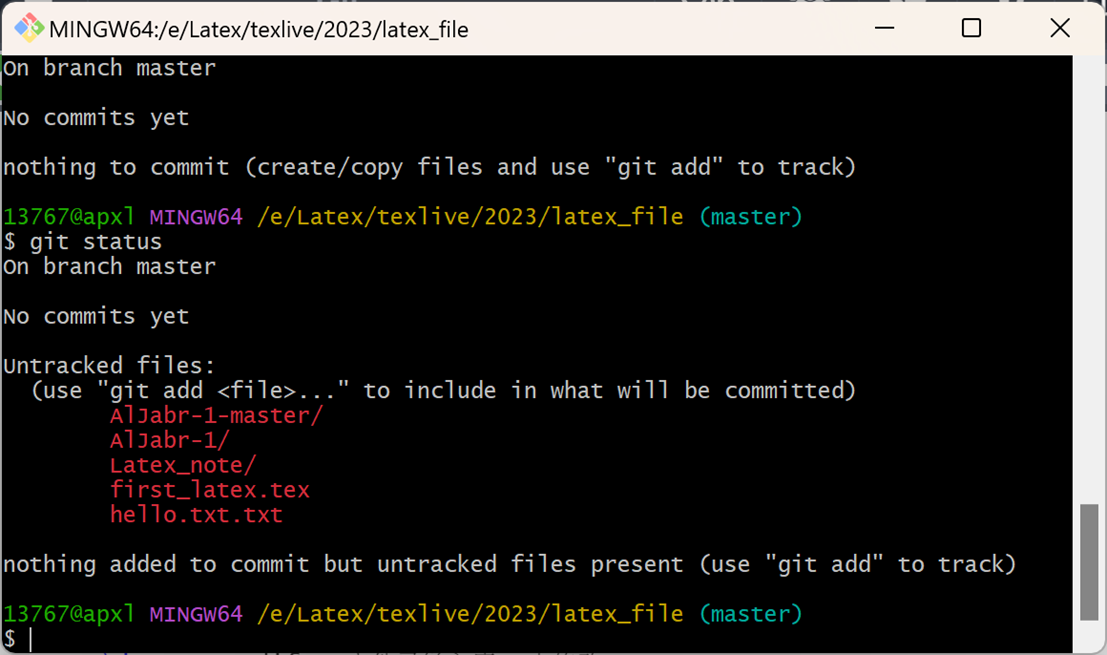
\includegraphics{image/9.1.png}

添加所有文件到暂存区: git add .
提交暂存区中的内容到本地仓库: git commit -m “文件名”, -m为提交信息

忽略文件:有些时候我们不想把某些文件纳入版本控制中,比如数据库文件,临时文件,设计文件等, 在主目录下建立".gitignore"文件,此文件有如下规则:
\begin{enumerate}
    \item 忽略文件中的空行或以井号(\verb|#|)开始的行将会被忽略,即为注释
    \item 可以使用Linux通配符。例如:星号(*)代表任意多个字符,(直接写一个*表示忽略所有内容),问号(?)代表一个字符,方括号([abc])代表可选字符范围,大括号({string1,string2,...})代表可选的字符串等
    \item 如果名称的最前面有一个感叹号(!),表示例外规则,将不被忽略
    \item 如果名称的最前面是一个路径分隔符(/),表示要忽略的文件在此目录下,而子目录中的文件不忽略(向上忽略)
    \item 如果名称的最后面是一个路径分隔符(/),表示要忽略的是此目录下该名称的子目录,而非文件(默认文件或目录都忽略)(向下忽略)
    \item \verb|[]|匹配一个字符列表,如a[mn]z可匹配amz和anz;**匹配多级目录,如a/**/b可匹配"a/b""a/x/b""a/x/y/b"
\end{enumerate}
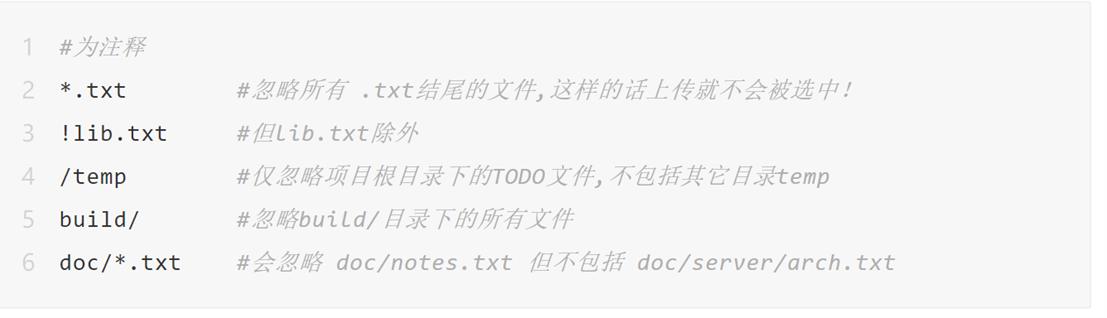
\includegraphics{image/9.2.png}

\section{配置SSH公钥及创建远程仓库}
\begin{flushleft}
(视频里用的码云,我用github,这里空了视频一章,此处的笔记是视频第十一章的东西)

点入电脑用户所在位置,此时应该没有.ssh文件:   
\end{flushleft}


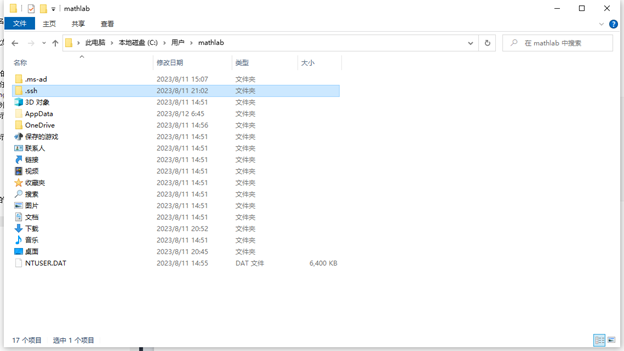
\includegraphics{image/10.1.png}

输入指令ssh-keygen -t rsa,一路回车可生成ssh密钥,一个公共的一个加密的:

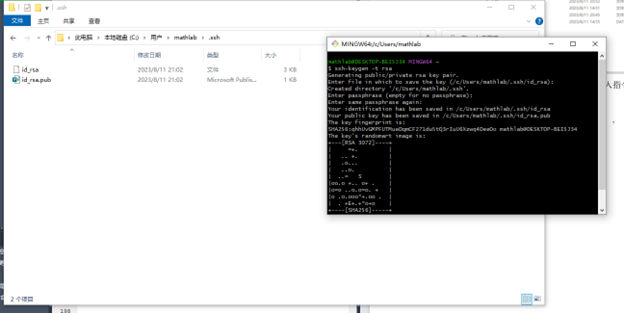
\includegraphics{image/10.2.png}
\begin{flushleft}
把公共ssh(文件小的那个)里面的复制进GitHub相关位置,标题起成自己邮箱名(密钥最后有写): 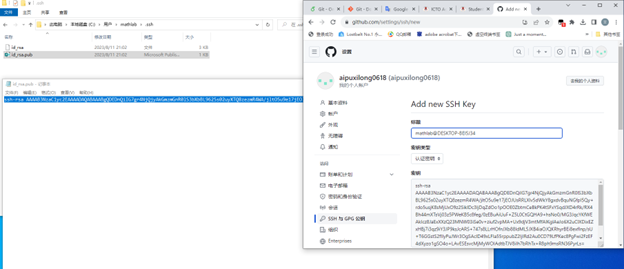
\includegraphics{image/10.3.png}

搞定!  

另注:从零开始从建库到远程克隆的完整操作:
\end{flushleft}

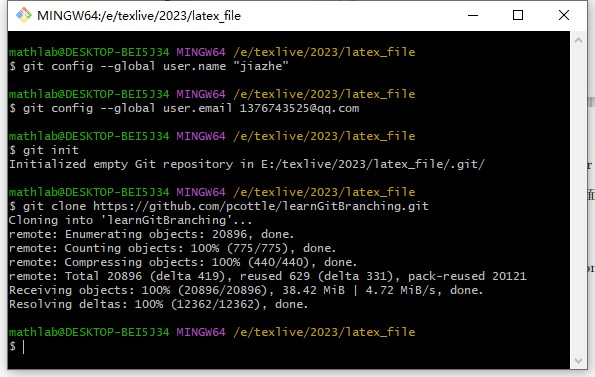
\includegraphics{image/图片1.jpg}

\section{分支管理与操作}
直接看图吧:
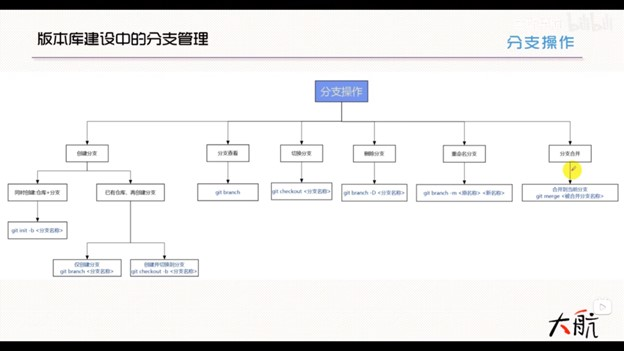
\includegraphics{image/11.1.jpg}

\section{实战操作及遇到的问题}
\begin{enumerate}
\item 打开一个新的文件夹:
\begin{lstlisting}[breaklines=true]
	git config --global user.name "jiazhe" %配置用户名及邮箱
	git config --global user.email 1376743525@qq.com
	
	git init %创建新的仓库,输入后会出现一个.git的隐藏文件
	git init -b 分支名称 %创建新的仓库并直接命名分支名称,个人觉得这么写更好,否则可能你本地默认一个master分支远程是个main分支,push后显示两个分支,还要合并删除啥的太麻烦
\end{lstlisting}

\item 克隆远程:
\begin{lstlisting}[breaklines=true]
	git clone 网页链接  %github里可以直接提取链接
\end{lstlisting}	
	
\item 本地文件相关代码:
\begin{lstlisting}[breaklines=true]
	git status %查看所有文件状态,有事没事就看看
	git add .  %添加到暂存区,.表示上传全部文件,也可以指定文件
	git commit %这么写会出来一个框,在vi编辑器里面写注释,i开始写写完后按esc键后:wq退出q!不保存退出
	git commit -m "提交的信息"  %也可以直接git commit --amend -m "提交的信息",查看日志里少一条
	
\end{lstlisting}	

\item 分支相关,因为我在这各种折腾所以代码相对较多:
\begin{lstlisting}[breaklines=true]
	git branch 分支名字  %创建本地分支
	git remote -v  %查看本地库对应的远程库
	git branch  %查看本地分支(对应当前分支有一个星号,正常是有输出的,未commit提交的库是空的,此时无显示,git add .以及git commit -m ""后就有显示了)
	git checkout 分支名称  %分支切换
	
				
\end{lstlisting}

\item 推送相关:
\begin{lstlisting}[breaklines=true]
	git remote add 远程库名称(自己起的名字) 远程库地址(网页的链接,直接复制)  %关联远程仓库,其实如果你建立库的时候啥也没有。它会提示你要干啥的。我就因为输代码的时候忘了add纠结了很久。。。。
	git branch -a  %列出所有(远端+近端)分支
	git push 远程库名称 分支名称 (推送所有:--all)  :向远程库推送本地分支
	git push   %先配置好远程才行,否则得输入github的用户名密码,第一次提交需要: git push -u 远程库名称 上传的分支  才行
\end{lstlisting}

\item 其他用到的代码:
\begin{lstlisting}
	git branch -d 分支名称  %删除分支
	git push 远程库名称 -d(-D:强制删除有修改未合并) 分支名称  %删除远程分支
	git remote remove 远程仓库名字  %移除已关联的远程仓库
\end{lstlisting}
在(乱删分支后)遇到过一个问题:failed to push some refs to 'https://github.com/aipuxilong0618/try-for-re
mote-connection.git' ,\href{https://www.cnblogs.com/Rainingday/p/12364690.html}{这是原因},用git pull --rebase origin main
可以搞定,再git push -u origin main就好
\end{enumerate}

\end{document}
